\documentclass[twoside]{book}

% Packages required by doxygen
\usepackage{fixltx2e}
\usepackage{calc}
\usepackage{doxygen}
\usepackage[export]{adjustbox} % also loads graphicx
\usepackage{graphicx}
\usepackage[utf8]{inputenc}
\usepackage{makeidx}
\usepackage{multicol}
\usepackage{multirow}
\PassOptionsToPackage{warn}{textcomp}
\usepackage{textcomp}
\usepackage[nointegrals]{wasysym}
\usepackage[table]{xcolor}

% Font selection
\usepackage[T1]{fontenc}
\usepackage[scaled=.90]{helvet}
\usepackage{courier}
\usepackage{amssymb}
\usepackage{sectsty}
\renewcommand{\familydefault}{\sfdefault}
\allsectionsfont{%
  \fontseries{bc}\selectfont%
  \color{darkgray}%
}
\renewcommand{\DoxyLabelFont}{%
  \fontseries{bc}\selectfont%
  \color{darkgray}%
}
\newcommand{\+}{\discretionary{\mbox{\scriptsize$\hookleftarrow$}}{}{}}

% Page & text layout
\usepackage{geometry}
\geometry{%
  a4paper,%
  top=2.5cm,%
  bottom=2.5cm,%
  left=2.5cm,%
  right=2.5cm%
}
\tolerance=750
\hfuzz=15pt
\hbadness=750
\setlength{\emergencystretch}{15pt}
\setlength{\parindent}{0cm}
\setlength{\parskip}{3ex plus 2ex minus 2ex}
\makeatletter
\renewcommand{\paragraph}{%
  \@startsection{paragraph}{4}{0ex}{-1.0ex}{1.0ex}{%
    \normalfont\normalsize\bfseries\SS@parafont%
  }%
}
\renewcommand{\subparagraph}{%
  \@startsection{subparagraph}{5}{0ex}{-1.0ex}{1.0ex}{%
    \normalfont\normalsize\bfseries\SS@subparafont%
  }%
}
\makeatother

% Headers & footers
\usepackage{fancyhdr}
\pagestyle{fancyplain}
\fancyhead[LE]{\fancyplain{}{\bfseries\thepage}}
\fancyhead[CE]{\fancyplain{}{}}
\fancyhead[RE]{\fancyplain{}{\bfseries\leftmark}}
\fancyhead[LO]{\fancyplain{}{\bfseries\rightmark}}
\fancyhead[CO]{\fancyplain{}{}}
\fancyhead[RO]{\fancyplain{}{\bfseries\thepage}}
\fancyfoot[LE]{\fancyplain{}{}}
\fancyfoot[CE]{\fancyplain{}{}}
\fancyfoot[RE]{\fancyplain{}{\bfseries\scriptsize Generated by Doxygen }}
\fancyfoot[LO]{\fancyplain{}{\bfseries\scriptsize Generated by Doxygen }}
\fancyfoot[CO]{\fancyplain{}{}}
\fancyfoot[RO]{\fancyplain{}{}}
\renewcommand{\footrulewidth}{0.4pt}
\renewcommand{\chaptermark}[1]{%
  \markboth{#1}{}%
}
\renewcommand{\sectionmark}[1]{%
  \markright{\thesection\ #1}%
}

% Indices & bibliography
\usepackage{natbib}
\usepackage[titles]{tocloft}
\setcounter{tocdepth}{3}
\setcounter{secnumdepth}{5}
\makeindex

% Hyperlinks (required, but should be loaded last)
\usepackage{ifpdf}
\ifpdf
  \usepackage[pdftex,pagebackref=true]{hyperref}
\else
  \usepackage[ps2pdf,pagebackref=true]{hyperref}
\fi
\hypersetup{%
  colorlinks=true,%
  linkcolor=blue,%
  citecolor=blue,%
  unicode%
}

% Custom commands
\newcommand{\clearemptydoublepage}{%
  \newpage{\pagestyle{empty}\cleardoublepage}%
}

\usepackage{caption}
\captionsetup{labelsep=space,justification=centering,font={bf},singlelinecheck=off,skip=4pt,position=top}

%===== C O N T E N T S =====

\begin{document}

% Titlepage & ToC
\hypersetup{pageanchor=false,
             bookmarksnumbered=true,
             pdfencoding=unicode
            }
\pagenumbering{alph}
\begin{titlepage}
\vspace*{7cm}
\begin{center}%
{\Large My Project }\\
\vspace*{1cm}
{\large Generated by Doxygen 1.8.13}\\
\end{center}
\end{titlepage}
\clearemptydoublepage
\pagenumbering{roman}
\tableofcontents
\clearemptydoublepage
\pagenumbering{arabic}
\hypersetup{pageanchor=true}

%--- Begin generated contents ---
\chapter{Hierarchical Index}
\section{Class Hierarchy}
This inheritance list is sorted roughly, but not completely, alphabetically\+:\begin{DoxyCompactList}
\item Exception\begin{DoxyCompactList}
\item \contentsline{section}{swimmypractice5.\+Check\+Exception}{\pageref{classswimmypractice5_1_1_check_exception}}{}
\end{DoxyCompactList}
\item \contentsline{section}{swimmypractice5.\+Main}{\pageref{classswimmypractice5_1_1_main}}{}
\item \contentsline{section}{swimmypractice5.\+Mobile\+Shop}{\pageref{classswimmypractice5_1_1_mobile_shop}}{}
\item \contentsline{section}{swimmypractice5.\+Smartphone}{\pageref{classswimmypractice5_1_1_smartphone}}{}
\begin{DoxyCompactList}
\item \contentsline{section}{swimmypractice5.\+Android}{\pageref{classswimmypractice5_1_1_android}}{}
\begin{DoxyCompactList}
\item \contentsline{section}{swimmypractice5.\+Aquos}{\pageref{classswimmypractice5_1_1_aquos}}{}
\item \contentsline{section}{swimmypractice5.\+Nexus}{\pageref{classswimmypractice5_1_1_nexus}}{}
\item \contentsline{section}{swimmypractice5.\+Xperia}{\pageref{classswimmypractice5_1_1_xperia}}{}
\end{DoxyCompactList}
\item \contentsline{section}{swimmypractice5.\+Iphone}{\pageref{classswimmypractice5_1_1_iphone}}{}
\begin{DoxyCompactList}
\item \contentsline{section}{swimmypractice5.\+Iphone6S}{\pageref{classswimmypractice5_1_1_iphone6_s}}{}
\item \contentsline{section}{swimmypractice5.\+Iphone7}{\pageref{classswimmypractice5_1_1_iphone7}}{}
\item \contentsline{section}{swimmypractice5.\+Iphone7plus}{\pageref{classswimmypractice5_1_1_iphone7plus}}{}
\end{DoxyCompactList}
\end{DoxyCompactList}
\end{DoxyCompactList}

\chapter{Class Index}
\section{Class List}
Here are the classes, structs, unions and interfaces with brief descriptions\+:\begin{DoxyCompactList}
\item\contentsline{section}{\hyperlink{classswimmypractice5_1_1_android}{swimmypractice5.\+Android} }{\pageref{classswimmypractice5_1_1_android}}{}
\item\contentsline{section}{\hyperlink{classswimmypractice5_1_1_aquos}{swimmypractice5.\+Aquos} }{\pageref{classswimmypractice5_1_1_aquos}}{}
\item\contentsline{section}{\hyperlink{classswimmypractice5_1_1_check_exception}{swimmypractice5.\+Check\+Exception} }{\pageref{classswimmypractice5_1_1_check_exception}}{}
\item\contentsline{section}{\hyperlink{classswimmypractice5_1_1_iphone}{swimmypractice5.\+Iphone} }{\pageref{classswimmypractice5_1_1_iphone}}{}
\item\contentsline{section}{\hyperlink{classswimmypractice5_1_1_iphone6_s}{swimmypractice5.\+Iphone6S} }{\pageref{classswimmypractice5_1_1_iphone6_s}}{}
\item\contentsline{section}{\hyperlink{classswimmypractice5_1_1_iphone7}{swimmypractice5.\+Iphone7} }{\pageref{classswimmypractice5_1_1_iphone7}}{}
\item\contentsline{section}{\hyperlink{classswimmypractice5_1_1_iphone7plus}{swimmypractice5.\+Iphone7plus} }{\pageref{classswimmypractice5_1_1_iphone7plus}}{}
\item\contentsline{section}{\hyperlink{classswimmypractice5_1_1_main}{swimmypractice5.\+Main} }{\pageref{classswimmypractice5_1_1_main}}{}
\item\contentsline{section}{\hyperlink{classswimmypractice5_1_1_mobile_shop}{swimmypractice5.\+Mobile\+Shop} }{\pageref{classswimmypractice5_1_1_mobile_shop}}{}
\item\contentsline{section}{\hyperlink{classswimmypractice5_1_1_nexus}{swimmypractice5.\+Nexus} }{\pageref{classswimmypractice5_1_1_nexus}}{}
\item\contentsline{section}{\hyperlink{classswimmypractice5_1_1_smartphone}{swimmypractice5.\+Smartphone} }{\pageref{classswimmypractice5_1_1_smartphone}}{}
\item\contentsline{section}{\hyperlink{classswimmypractice5_1_1_xperia}{swimmypractice5.\+Xperia} }{\pageref{classswimmypractice5_1_1_xperia}}{}
\end{DoxyCompactList}

\chapter{Class Documentation}
\hypertarget{classswimmypractice5_1_1_android}{}\section{swimmypractice5.\+Android Class Reference}
\label{classswimmypractice5_1_1_android}\index{swimmypractice5.\+Android@{swimmypractice5.\+Android}}
Inheritance diagram for swimmypractice5.\+Android\+:\begin{figure}[H]
\begin{center}
\leavevmode
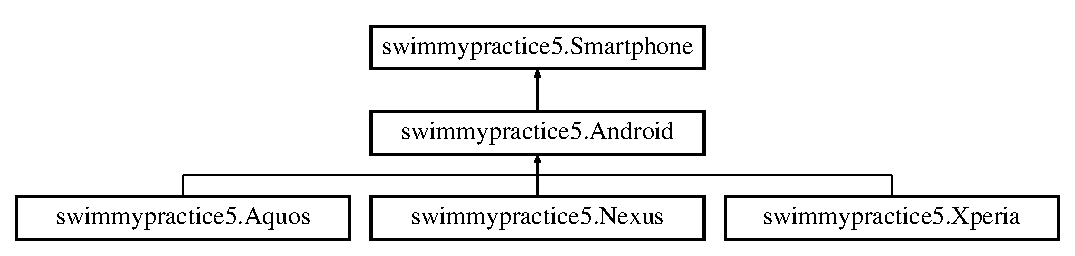
\includegraphics[height=2.994653cm]{classswimmypractice5_1_1_android}
\end{center}
\end{figure}
\subsection*{Public Member Functions}
\begin{DoxyCompactItemize}
\item 
\mbox{\Hypertarget{classswimmypractice5_1_1_android_a703e09e859a662d5388651e1b1f8664d}\label{classswimmypractice5_1_1_android_a703e09e859a662d5388651e1b1f8664d}} 
{\bfseries Android} (String a\+Name)
\item 
\mbox{\Hypertarget{classswimmypractice5_1_1_android_a3b33d85566b829f421c023fcdf91aef7}\label{classswimmypractice5_1_1_android_a3b33d85566b829f421c023fcdf91aef7}} 
void {\bfseries music} ()  throws Check\+Exception
\end{DoxyCompactItemize}
\subsection*{Additional Inherited Members}


The documentation for this class was generated from the following file\+:\begin{DoxyCompactItemize}
\item 
Android.\+java\end{DoxyCompactItemize}

\hypertarget{classswimmypractice5_1_1_aquos}{}\section{swimmypractice5.\+Aquos Class Reference}
\label{classswimmypractice5_1_1_aquos}\index{swimmypractice5.\+Aquos@{swimmypractice5.\+Aquos}}
Inheritance diagram for swimmypractice5.\+Aquos\+:\begin{figure}[H]
\begin{center}
\leavevmode
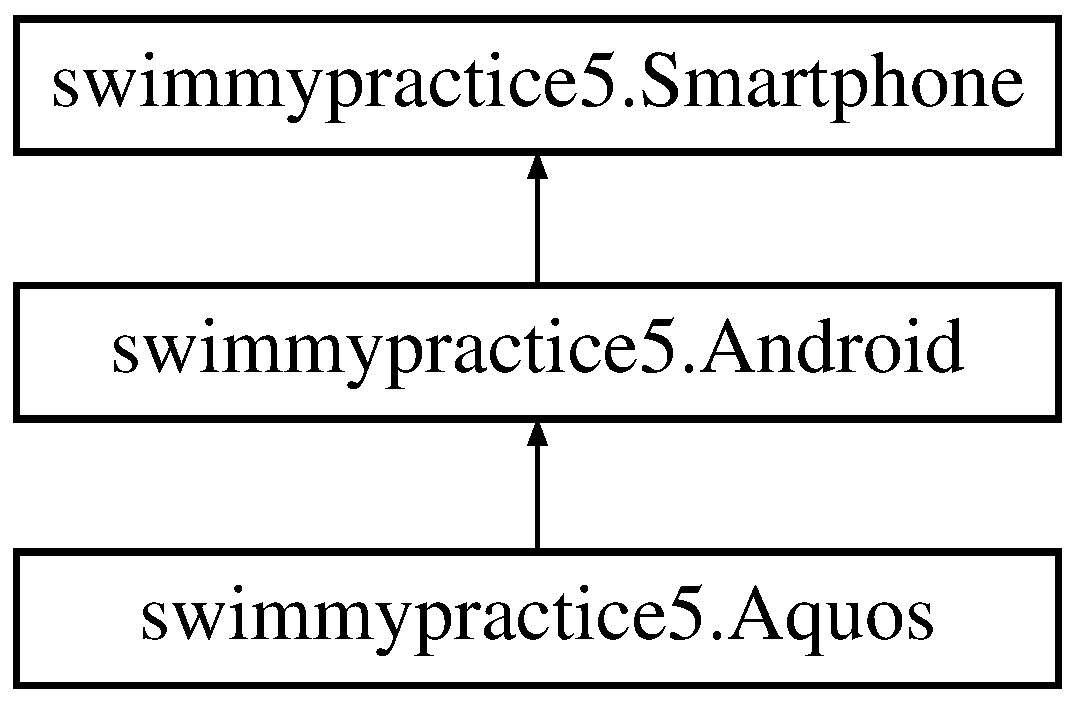
\includegraphics[height=3.000000cm]{classswimmypractice5_1_1_aquos}
\end{center}
\end{figure}
\subsection*{Public Member Functions}
\begin{DoxyCompactItemize}
\item 
\mbox{\Hypertarget{classswimmypractice5_1_1_aquos_a4b5725ac1e46c683b0e37c4b1b103241}\label{classswimmypractice5_1_1_aquos_a4b5725ac1e46c683b0e37c4b1b103241}} 
void {\bfseries send\+Mail} ()  throws Check\+Exception
\end{DoxyCompactItemize}
\subsection*{Additional Inherited Members}


The documentation for this class was generated from the following file\+:\begin{DoxyCompactItemize}
\item 
Aquos.\+java\end{DoxyCompactItemize}

\hypertarget{classswimmypractice5_1_1_check_exception}{}\section{swimmypractice5.\+Check\+Exception Class Reference}
\label{classswimmypractice5_1_1_check_exception}\index{swimmypractice5.\+Check\+Exception@{swimmypractice5.\+Check\+Exception}}
Inheritance diagram for swimmypractice5.\+Check\+Exception\+:\begin{figure}[H]
\begin{center}
\leavevmode
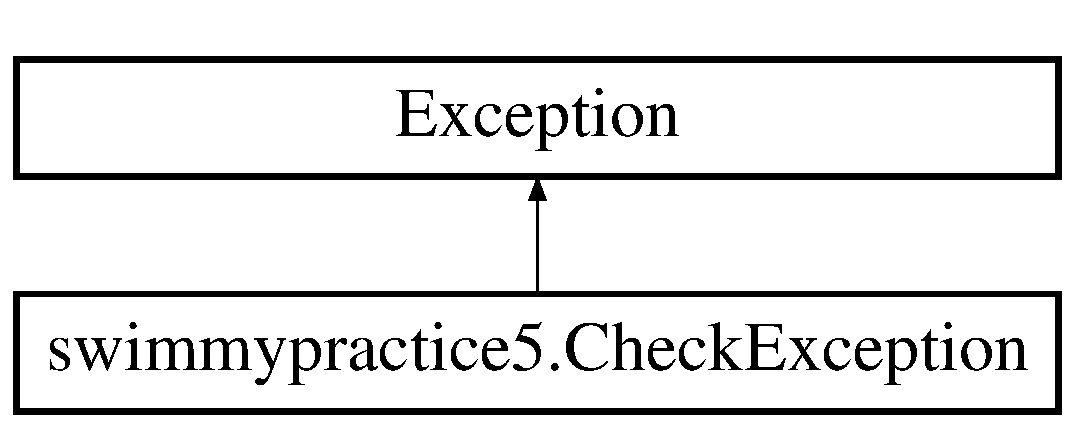
\includegraphics[height=2.000000cm]{classswimmypractice5_1_1_check_exception}
\end{center}
\end{figure}
\subsection*{Public Member Functions}
\begin{DoxyCompactItemize}
\item 
\mbox{\Hypertarget{classswimmypractice5_1_1_check_exception_a013350058bc8498f16e0381afa7059f2}\label{classswimmypractice5_1_1_check_exception_a013350058bc8498f16e0381afa7059f2}} 
{\bfseries Check\+Exception} (String str)
\end{DoxyCompactItemize}


The documentation for this class was generated from the following file\+:\begin{DoxyCompactItemize}
\item 
Check\+Exception.\+java\end{DoxyCompactItemize}

\hypertarget{classswimmypractice5_1_1_iphone}{}\section{swimmypractice5.\+Iphone Class Reference}
\label{classswimmypractice5_1_1_iphone}\index{swimmypractice5.\+Iphone@{swimmypractice5.\+Iphone}}
Inheritance diagram for swimmypractice5.\+Iphone\+:\begin{figure}[H]
\begin{center}
\leavevmode
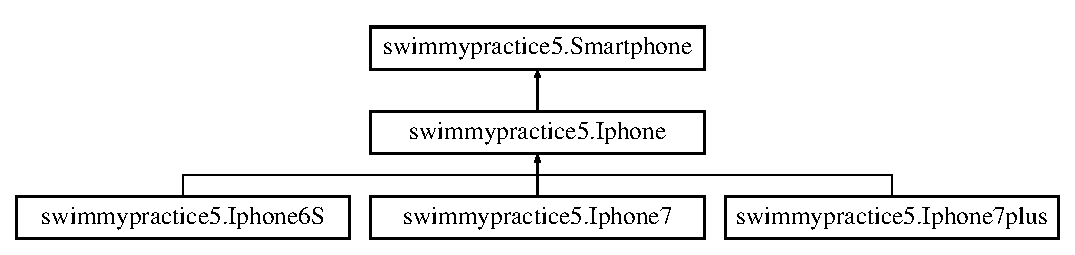
\includegraphics[height=2.978723cm]{classswimmypractice5_1_1_iphone}
\end{center}
\end{figure}
\subsection*{Public Member Functions}
\begin{DoxyCompactItemize}
\item 
\mbox{\Hypertarget{classswimmypractice5_1_1_iphone_acf7e3a44e1ae4bbe648b88fd9fde4766}\label{classswimmypractice5_1_1_iphone_acf7e3a44e1ae4bbe648b88fd9fde4766}} 
{\bfseries Iphone} (String a\+Name)
\item 
\mbox{\Hypertarget{classswimmypractice5_1_1_iphone_a375d7b0bc7c61f14b6a692b0c760187d}\label{classswimmypractice5_1_1_iphone_a375d7b0bc7c61f14b6a692b0c760187d}} 
void {\bfseries music} ()  throws Check\+Exception 
\end{DoxyCompactItemize}
\subsection*{Additional Inherited Members}


The documentation for this class was generated from the following file\+:\begin{DoxyCompactItemize}
\item 
Iphone.\+java\end{DoxyCompactItemize}

\hypertarget{classswimmypractice5_1_1_iphone6_s}{}\section{swimmypractice5.\+Iphone6S Class Reference}
\label{classswimmypractice5_1_1_iphone6_s}\index{swimmypractice5.\+Iphone6S@{swimmypractice5.\+Iphone6S}}
Inheritance diagram for swimmypractice5.\+Iphone6S\+:\begin{figure}[H]
\begin{center}
\leavevmode
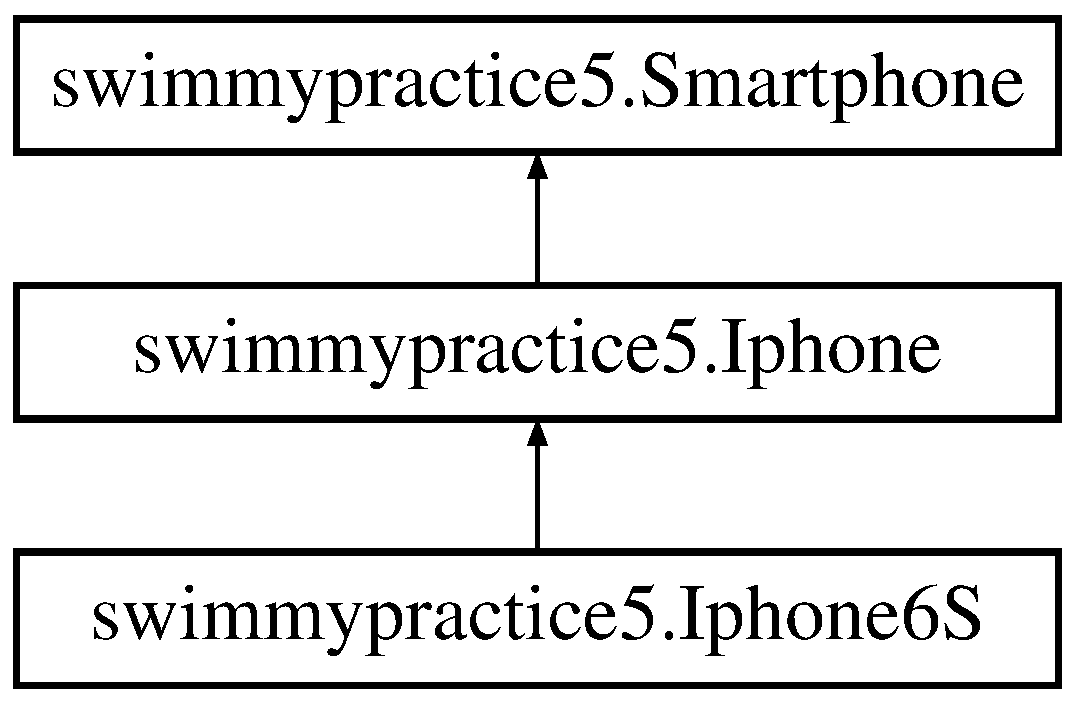
\includegraphics[height=3.000000cm]{classswimmypractice5_1_1_iphone6_s}
\end{center}
\end{figure}
\subsection*{Public Member Functions}
\begin{DoxyCompactItemize}
\item 
\mbox{\Hypertarget{classswimmypractice5_1_1_iphone6_s_a6bfff10d4ae15856a03dddb10dcb4cfd}\label{classswimmypractice5_1_1_iphone6_s_a6bfff10d4ae15856a03dddb10dcb4cfd}} 
void {\bfseries send\+Mail} ()  throws Check\+Exception
\end{DoxyCompactItemize}
\subsection*{Additional Inherited Members}


The documentation for this class was generated from the following file\+:\begin{DoxyCompactItemize}
\item 
Iphone6\+S.\+java\end{DoxyCompactItemize}

\hypertarget{classswimmypractice5_1_1_iphone7}{}\section{swimmypractice5.\+Iphone7 Class Reference}
\label{classswimmypractice5_1_1_iphone7}\index{swimmypractice5.\+Iphone7@{swimmypractice5.\+Iphone7}}
Inheritance diagram for swimmypractice5.\+Iphone7\+:\begin{figure}[H]
\begin{center}
\leavevmode
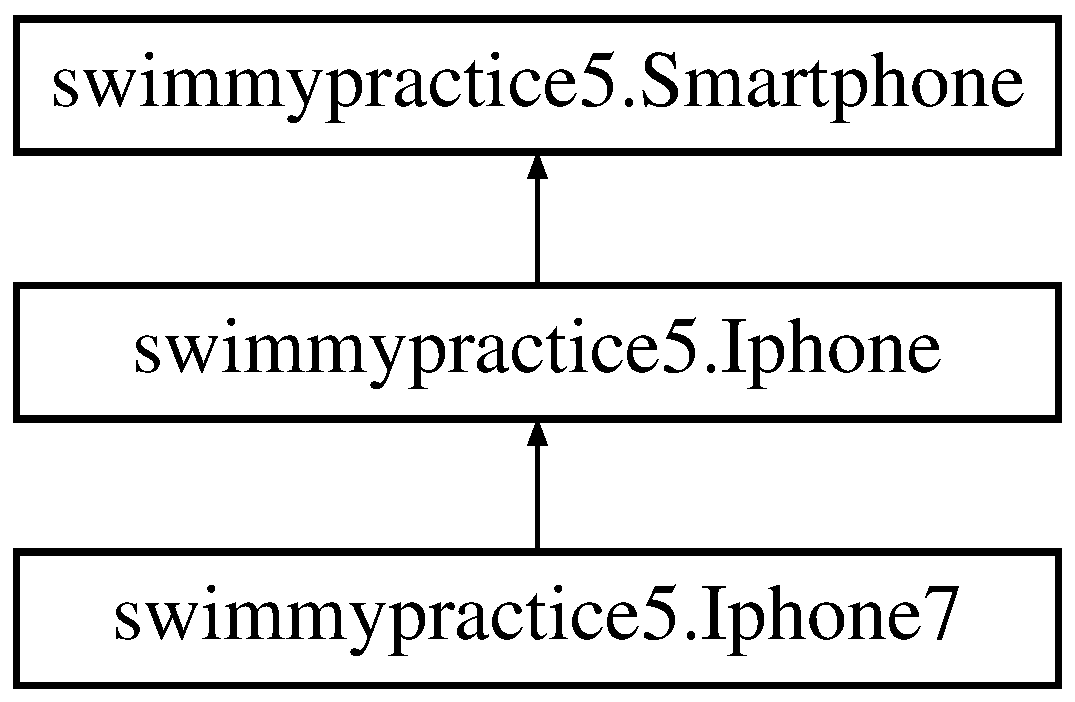
\includegraphics[height=3.000000cm]{classswimmypractice5_1_1_iphone7}
\end{center}
\end{figure}
\subsection*{Public Member Functions}
\begin{DoxyCompactItemize}
\item 
\mbox{\Hypertarget{classswimmypractice5_1_1_iphone7_a845c8fba41e6428531e313c34d34a546}\label{classswimmypractice5_1_1_iphone7_a845c8fba41e6428531e313c34d34a546}} 
void {\bfseries send\+Mail} ()  throws Check\+Exception
\end{DoxyCompactItemize}
\subsection*{Additional Inherited Members}


The documentation for this class was generated from the following file\+:\begin{DoxyCompactItemize}
\item 
Iphone7.\+java\end{DoxyCompactItemize}

\hypertarget{classswimmypractice5_1_1_iphone7plus}{}\section{swimmypractice5.\+Iphone7plus Class Reference}
\label{classswimmypractice5_1_1_iphone7plus}\index{swimmypractice5.\+Iphone7plus@{swimmypractice5.\+Iphone7plus}}
Inheritance diagram for swimmypractice5.\+Iphone7plus\+:\begin{figure}[H]
\begin{center}
\leavevmode
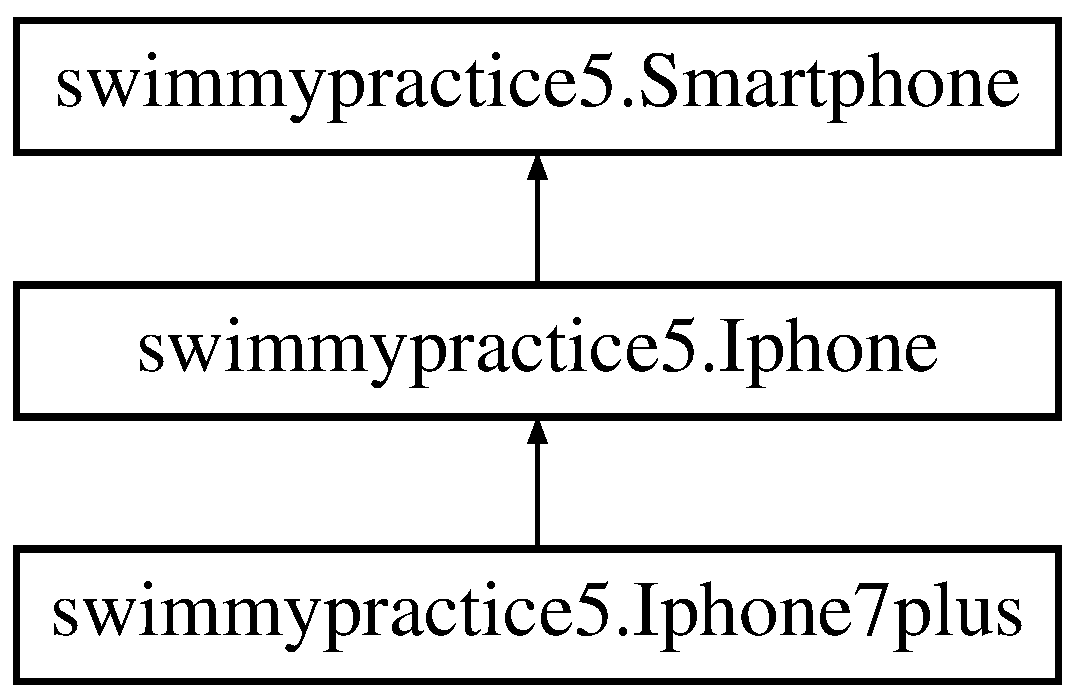
\includegraphics[height=3.000000cm]{classswimmypractice5_1_1_iphone7plus}
\end{center}
\end{figure}
\subsection*{Public Member Functions}
\begin{DoxyCompactItemize}
\item 
\mbox{\Hypertarget{classswimmypractice5_1_1_iphone7plus_a1c5399c99a122551b7f8fee9bc4b56c1}\label{classswimmypractice5_1_1_iphone7plus_a1c5399c99a122551b7f8fee9bc4b56c1}} 
void {\bfseries send\+Mail} ()  throws Check\+Exception
\end{DoxyCompactItemize}
\subsection*{Additional Inherited Members}


The documentation for this class was generated from the following file\+:\begin{DoxyCompactItemize}
\item 
Iphone7plus.\+java\end{DoxyCompactItemize}

\hypertarget{classswimmypractice5_1_1_main}{}\section{swimmypractice5.\+Main Class Reference}
\label{classswimmypractice5_1_1_main}\index{swimmypractice5.\+Main@{swimmypractice5.\+Main}}
\subsection*{Static Public Member Functions}
\begin{DoxyCompactItemize}
\item 
\mbox{\Hypertarget{classswimmypractice5_1_1_main_a7b62064a97d750db92bed427b7d5324d}\label{classswimmypractice5_1_1_main_a7b62064a97d750db92bed427b7d5324d}} 
static void {\bfseries main} (String\mbox{[}$\,$\mbox{]} args)  throws Exception 
\end{DoxyCompactItemize}


The documentation for this class was generated from the following file\+:\begin{DoxyCompactItemize}
\item 
Main.\+java\end{DoxyCompactItemize}

\hypertarget{classswimmypractice5_1_1_mobile_shop}{}\section{swimmypractice5.\+Mobile\+Shop Class Reference}
\label{classswimmypractice5_1_1_mobile_shop}\index{swimmypractice5.\+Mobile\+Shop@{swimmypractice5.\+Mobile\+Shop}}
\subsection*{Public Member Functions}
\begin{DoxyCompactItemize}
\item 
\mbox{\Hypertarget{classswimmypractice5_1_1_mobile_shop_ac1e379aee7909f1fbfbd9e2b82a033d5}\label{classswimmypractice5_1_1_mobile_shop_ac1e379aee7909f1fbfbd9e2b82a033d5}} 
\hyperlink{classswimmypractice5_1_1_iphone}{Iphone} {\bfseries choice\+Iphone} ()
\item 
\mbox{\Hypertarget{classswimmypractice5_1_1_mobile_shop_acb06ee43812e6046754c5628ba74c01e}\label{classswimmypractice5_1_1_mobile_shop_acb06ee43812e6046754c5628ba74c01e}} 
\hyperlink{classswimmypractice5_1_1_android}{Android} {\bfseries choice\+Android} ()
\end{DoxyCompactItemize}


The documentation for this class was generated from the following file\+:\begin{DoxyCompactItemize}
\item 
Mobile\+Shop.\+java\end{DoxyCompactItemize}

\hypertarget{classswimmypractice5_1_1_nexus}{}\section{swimmypractice5.\+Nexus Class Reference}
\label{classswimmypractice5_1_1_nexus}\index{swimmypractice5.\+Nexus@{swimmypractice5.\+Nexus}}
Inheritance diagram for swimmypractice5.\+Nexus\+:\begin{figure}[H]
\begin{center}
\leavevmode
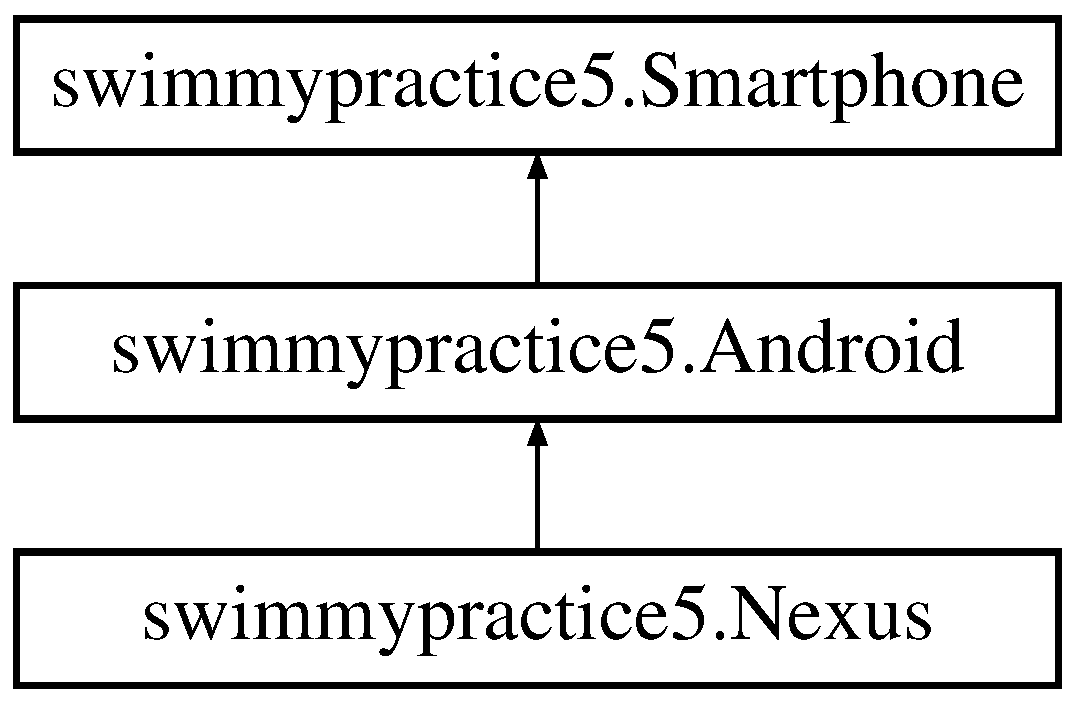
\includegraphics[height=3.000000cm]{classswimmypractice5_1_1_nexus}
\end{center}
\end{figure}
\subsection*{Public Member Functions}
\begin{DoxyCompactItemize}
\item 
\mbox{\Hypertarget{classswimmypractice5_1_1_nexus_aa66d609fa43e982eb92d528656225765}\label{classswimmypractice5_1_1_nexus_aa66d609fa43e982eb92d528656225765}} 
void {\bfseries send\+Mail} ()  throws Check\+Exception 
\end{DoxyCompactItemize}
\subsection*{Additional Inherited Members}


The documentation for this class was generated from the following file\+:\begin{DoxyCompactItemize}
\item 
Nexus.\+java\end{DoxyCompactItemize}

\hypertarget{classswimmypractice5_1_1_smartphone}{}\section{swimmypractice5.\+Smartphone Class Reference}
\label{classswimmypractice5_1_1_smartphone}\index{swimmypractice5.\+Smartphone@{swimmypractice5.\+Smartphone}}
Inheritance diagram for swimmypractice5.\+Smartphone\+:\begin{figure}[H]
\begin{center}
\leavevmode
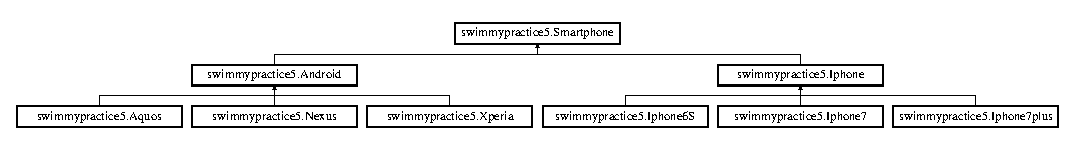
\includegraphics[height=1.489362cm]{classswimmypractice5_1_1_smartphone}
\end{center}
\end{figure}
\subsection*{Classes}
\begin{DoxyCompactItemize}
\item 
enum {\bfseries Smartphone\+Kind}
\end{DoxyCompactItemize}
\subsection*{Public Member Functions}
\begin{DoxyCompactItemize}
\item 
\mbox{\Hypertarget{classswimmypractice5_1_1_smartphone_aa653b938902784088470a3f0703feefe}\label{classswimmypractice5_1_1_smartphone_aa653b938902784088470a3f0703feefe}} 
{\bfseries Smartphone} (Smartphone\+Kind a\+Kind, String a\+Name)
\item 
\mbox{\Hypertarget{classswimmypractice5_1_1_smartphone_a16bffc9a4a730adc571a4ddfdb9e9e4c}\label{classswimmypractice5_1_1_smartphone_a16bffc9a4a730adc571a4ddfdb9e9e4c}} 
Smartphone\+Kind {\bfseries get\+Kind} ()
\item 
\mbox{\Hypertarget{classswimmypractice5_1_1_smartphone_af1d4cedfc2937ec4c8c81d858a917ef7}\label{classswimmypractice5_1_1_smartphone_af1d4cedfc2937ec4c8c81d858a917ef7}} 
void {\bfseries input\+And\+Set\+Kind} ()
\item 
\mbox{\Hypertarget{classswimmypractice5_1_1_smartphone_a58f2805dc48669aba850c6aa50c0b6b2}\label{classswimmypractice5_1_1_smartphone_a58f2805dc48669aba850c6aa50c0b6b2}} 
String {\bfseries get\+Cpu} ()
\item 
\mbox{\Hypertarget{classswimmypractice5_1_1_smartphone_a1f561d11d3d7d10c436677b88dfe30d7}\label{classswimmypractice5_1_1_smartphone_a1f561d11d3d7d10c436677b88dfe30d7}} 
void {\bfseries input\+And\+Set\+Cpu} ()
\item 
\mbox{\Hypertarget{classswimmypractice5_1_1_smartphone_a6d942717cede6f41daaca02d557dcfb3}\label{classswimmypractice5_1_1_smartphone_a6d942717cede6f41daaca02d557dcfb3}} 
int {\bfseries get\+Ram} ()
\item 
\mbox{\Hypertarget{classswimmypractice5_1_1_smartphone_a1b89c55326ba55ab332ae3e3a63492f4}\label{classswimmypractice5_1_1_smartphone_a1b89c55326ba55ab332ae3e3a63492f4}} 
void {\bfseries input\+And\+Set\+Ram} ()
\item 
\mbox{\Hypertarget{classswimmypractice5_1_1_smartphone_a5f8a1a80936ab416a072bd0edae4ef8d}\label{classswimmypractice5_1_1_smartphone_a5f8a1a80936ab416a072bd0edae4ef8d}} 
int {\bfseries get\+Rom} ()
\item 
\mbox{\Hypertarget{classswimmypractice5_1_1_smartphone_a66b2e5acbda4f97a49dbe32a299bc188}\label{classswimmypractice5_1_1_smartphone_a66b2e5acbda4f97a49dbe32a299bc188}} 
void {\bfseries input\+And\+Set\+Rom} ()
\item 
\mbox{\Hypertarget{classswimmypractice5_1_1_smartphone_a8b6d550030d179ee09856ccac44ee348}\label{classswimmypractice5_1_1_smartphone_a8b6d550030d179ee09856ccac44ee348}} 
void {\bfseries send\+Mail} ()  throws Check\+Exception
\item 
\mbox{\Hypertarget{classswimmypractice5_1_1_smartphone_a6132726ae6e1d135a784fa59a27575b9}\label{classswimmypractice5_1_1_smartphone_a6132726ae6e1d135a784fa59a27575b9}} 
void {\bfseries music} ()  throws Check\+Exception  
\item 
\mbox{\Hypertarget{classswimmypractice5_1_1_smartphone_aa41ab0fe3d572d360d2d7068233aba91}\label{classswimmypractice5_1_1_smartphone_aa41ab0fe3d572d360d2d7068233aba91}} 
void {\bfseries tell} (int countrycode, String phonenumber)  throws Check\+Exception
\item 
\mbox{\Hypertarget{classswimmypractice5_1_1_smartphone_a80425c13cea1cb2b7ec50cb2e599759d}\label{classswimmypractice5_1_1_smartphone_a80425c13cea1cb2b7ec50cb2e599759d}} 
void {\bfseries tell} (int lineid)  throws Check\+Exception
\item 
\mbox{\Hypertarget{classswimmypractice5_1_1_smartphone_add498943a7c49d5caa8b0fee4e4e523b}\label{classswimmypractice5_1_1_smartphone_add498943a7c49d5caa8b0fee4e4e523b}} 
void {\bfseries check} ()  throws Check\+Exception
\end{DoxyCompactItemize}
\subsection*{Protected Attributes}
\begin{DoxyCompactItemize}
\item 
\mbox{\Hypertarget{classswimmypractice5_1_1_smartphone_aad0c3687814a221a2d1db8b8668416f5}\label{classswimmypractice5_1_1_smartphone_aad0c3687814a221a2d1db8b8668416f5}} 
Smartphone\+Kind {\bfseries Kind}
\item 
\mbox{\Hypertarget{classswimmypractice5_1_1_smartphone_a429a919aebb3a8a1495f2fbe0a7f0ad9}\label{classswimmypractice5_1_1_smartphone_a429a919aebb3a8a1495f2fbe0a7f0ad9}} 
String {\bfseries Name}
\item 
\mbox{\Hypertarget{classswimmypractice5_1_1_smartphone_ac6b3d91ad8c976fa50ced5075b65a915}\label{classswimmypractice5_1_1_smartphone_ac6b3d91ad8c976fa50ced5075b65a915}} 
String {\bfseries Cpu}
\item 
\mbox{\Hypertarget{classswimmypractice5_1_1_smartphone_ab5d518cc00d902934360b8c902e894df}\label{classswimmypractice5_1_1_smartphone_ab5d518cc00d902934360b8c902e894df}} 
int {\bfseries Ram}
\item 
\mbox{\Hypertarget{classswimmypractice5_1_1_smartphone_a6afd722dff66d4649fdafb03ec9eb660}\label{classswimmypractice5_1_1_smartphone_a6afd722dff66d4649fdafb03ec9eb660}} 
int {\bfseries Rom}
\end{DoxyCompactItemize}


The documentation for this class was generated from the following file\+:\begin{DoxyCompactItemize}
\item 
Smartphone.\+java\end{DoxyCompactItemize}

\hypertarget{classswimmypractice5_1_1_xperia}{}\section{swimmypractice5.\+Xperia Class Reference}
\label{classswimmypractice5_1_1_xperia}\index{swimmypractice5.\+Xperia@{swimmypractice5.\+Xperia}}
Inheritance diagram for swimmypractice5.\+Xperia\+:\begin{figure}[H]
\begin{center}
\leavevmode
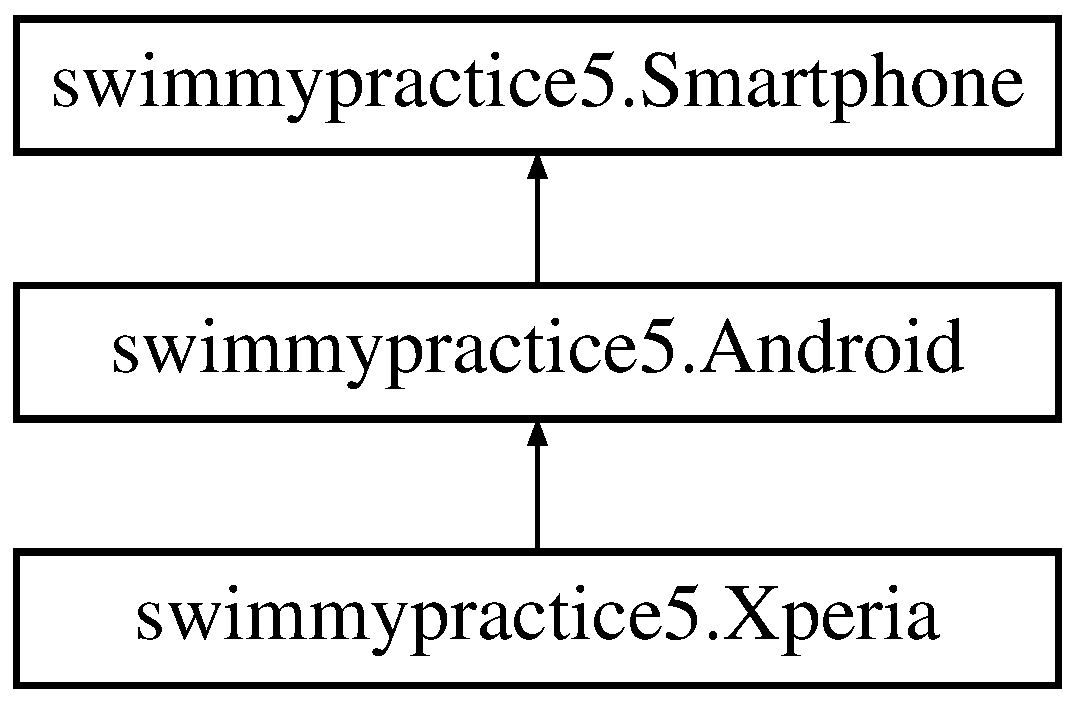
\includegraphics[height=3.000000cm]{classswimmypractice5_1_1_xperia}
\end{center}
\end{figure}
\subsection*{Public Member Functions}
\begin{DoxyCompactItemize}
\item 
\mbox{\Hypertarget{classswimmypractice5_1_1_xperia_a26c4b5fd95e2ca6ecd7f5c4d0a896f89}\label{classswimmypractice5_1_1_xperia_a26c4b5fd95e2ca6ecd7f5c4d0a896f89}} 
void {\bfseries send\+Mail} ()  throws Check\+Exception
\end{DoxyCompactItemize}
\subsection*{Additional Inherited Members}


The documentation for this class was generated from the following file\+:\begin{DoxyCompactItemize}
\item 
Xperia.\+java\end{DoxyCompactItemize}

%--- End generated contents ---

% Index
\backmatter
\newpage
\phantomsection
\clearemptydoublepage
\addcontentsline{toc}{chapter}{Index}
\printindex

\end{document}
